% Options for packages loaded elsewhere
\PassOptionsToPackage{unicode}{hyperref}
\PassOptionsToPackage{hyphens}{url}
%
\documentclass[
]{article}
\usepackage{lmodern}
\usepackage{amssymb,amsmath}
\usepackage{ifxetex,ifluatex}
\ifnum 0\ifxetex 1\fi\ifluatex 1\fi=0 % if pdftex
  \usepackage[T1]{fontenc}
  \usepackage[utf8]{inputenc}
  \usepackage{textcomp} % provide euro and other symbols
\else % if luatex or xetex
  \usepackage{unicode-math}
  \defaultfontfeatures{Scale=MatchLowercase}
  \defaultfontfeatures[\rmfamily]{Ligatures=TeX,Scale=1}
\fi
% Use upquote if available, for straight quotes in verbatim environments
\IfFileExists{upquote.sty}{\usepackage{upquote}}{}
\IfFileExists{microtype.sty}{% use microtype if available
  \usepackage[]{microtype}
  \UseMicrotypeSet[protrusion]{basicmath} % disable protrusion for tt fonts
}{}
\makeatletter
\@ifundefined{KOMAClassName}{% if non-KOMA class
  \IfFileExists{parskip.sty}{%
    \usepackage{parskip}
  }{% else
    \setlength{\parindent}{0pt}
    \setlength{\parskip}{6pt plus 2pt minus 1pt}}
}{% if KOMA class
  \KOMAoptions{parskip=half}}
\makeatother
\usepackage{xcolor}
\IfFileExists{xurl.sty}{\usepackage{xurl}}{} % add URL line breaks if available
\IfFileExists{bookmark.sty}{\usepackage{bookmark}}{\usepackage{hyperref}}
\hypersetup{
  pdftitle={Reproducible Research: Peer Assessment 1},
  hidelinks,
  pdfcreator={LaTeX via pandoc}}
\urlstyle{same} % disable monospaced font for URLs
\usepackage[margin=1in]{geometry}
\usepackage{color}
\usepackage{fancyvrb}
\newcommand{\VerbBar}{|}
\newcommand{\VERB}{\Verb[commandchars=\\\{\}]}
\DefineVerbatimEnvironment{Highlighting}{Verbatim}{commandchars=\\\{\}}
% Add ',fontsize=\small' for more characters per line
\usepackage{framed}
\definecolor{shadecolor}{RGB}{248,248,248}
\newenvironment{Shaded}{\begin{snugshade}}{\end{snugshade}}
\newcommand{\AlertTok}[1]{\textcolor[rgb]{0.94,0.16,0.16}{#1}}
\newcommand{\AnnotationTok}[1]{\textcolor[rgb]{0.56,0.35,0.01}{\textbf{\textit{#1}}}}
\newcommand{\AttributeTok}[1]{\textcolor[rgb]{0.77,0.63,0.00}{#1}}
\newcommand{\BaseNTok}[1]{\textcolor[rgb]{0.00,0.00,0.81}{#1}}
\newcommand{\BuiltInTok}[1]{#1}
\newcommand{\CharTok}[1]{\textcolor[rgb]{0.31,0.60,0.02}{#1}}
\newcommand{\CommentTok}[1]{\textcolor[rgb]{0.56,0.35,0.01}{\textit{#1}}}
\newcommand{\CommentVarTok}[1]{\textcolor[rgb]{0.56,0.35,0.01}{\textbf{\textit{#1}}}}
\newcommand{\ConstantTok}[1]{\textcolor[rgb]{0.00,0.00,0.00}{#1}}
\newcommand{\ControlFlowTok}[1]{\textcolor[rgb]{0.13,0.29,0.53}{\textbf{#1}}}
\newcommand{\DataTypeTok}[1]{\textcolor[rgb]{0.13,0.29,0.53}{#1}}
\newcommand{\DecValTok}[1]{\textcolor[rgb]{0.00,0.00,0.81}{#1}}
\newcommand{\DocumentationTok}[1]{\textcolor[rgb]{0.56,0.35,0.01}{\textbf{\textit{#1}}}}
\newcommand{\ErrorTok}[1]{\textcolor[rgb]{0.64,0.00,0.00}{\textbf{#1}}}
\newcommand{\ExtensionTok}[1]{#1}
\newcommand{\FloatTok}[1]{\textcolor[rgb]{0.00,0.00,0.81}{#1}}
\newcommand{\FunctionTok}[1]{\textcolor[rgb]{0.00,0.00,0.00}{#1}}
\newcommand{\ImportTok}[1]{#1}
\newcommand{\InformationTok}[1]{\textcolor[rgb]{0.56,0.35,0.01}{\textbf{\textit{#1}}}}
\newcommand{\KeywordTok}[1]{\textcolor[rgb]{0.13,0.29,0.53}{\textbf{#1}}}
\newcommand{\NormalTok}[1]{#1}
\newcommand{\OperatorTok}[1]{\textcolor[rgb]{0.81,0.36,0.00}{\textbf{#1}}}
\newcommand{\OtherTok}[1]{\textcolor[rgb]{0.56,0.35,0.01}{#1}}
\newcommand{\PreprocessorTok}[1]{\textcolor[rgb]{0.56,0.35,0.01}{\textit{#1}}}
\newcommand{\RegionMarkerTok}[1]{#1}
\newcommand{\SpecialCharTok}[1]{\textcolor[rgb]{0.00,0.00,0.00}{#1}}
\newcommand{\SpecialStringTok}[1]{\textcolor[rgb]{0.31,0.60,0.02}{#1}}
\newcommand{\StringTok}[1]{\textcolor[rgb]{0.31,0.60,0.02}{#1}}
\newcommand{\VariableTok}[1]{\textcolor[rgb]{0.00,0.00,0.00}{#1}}
\newcommand{\VerbatimStringTok}[1]{\textcolor[rgb]{0.31,0.60,0.02}{#1}}
\newcommand{\WarningTok}[1]{\textcolor[rgb]{0.56,0.35,0.01}{\textbf{\textit{#1}}}}
\usepackage{graphicx,grffile}
\makeatletter
\def\maxwidth{\ifdim\Gin@nat@width>\linewidth\linewidth\else\Gin@nat@width\fi}
\def\maxheight{\ifdim\Gin@nat@height>\textheight\textheight\else\Gin@nat@height\fi}
\makeatother
% Scale images if necessary, so that they will not overflow the page
% margins by default, and it is still possible to overwrite the defaults
% using explicit options in \includegraphics[width, height, ...]{}
\setkeys{Gin}{width=\maxwidth,height=\maxheight,keepaspectratio}
% Set default figure placement to htbp
\makeatletter
\def\fps@figure{htbp}
\makeatother
\setlength{\emergencystretch}{3em} % prevent overfull lines
\providecommand{\tightlist}{%
  \setlength{\itemsep}{0pt}\setlength{\parskip}{0pt}}
\setcounter{secnumdepth}{-\maxdimen} % remove section numbering

\title{Reproducible Research: Peer Assessment 1}
\author{}
\date{\vspace{-2.5em}}

\begin{document}
\maketitle

\hypertarget{introduction}{%
\subsection{Introduction}\label{introduction}}

Activity data is now easily collected via smart watches and other
athletic devices such as Fitbit and Nike Fuelband. The goal for this
project is to do data exploration to uncover the characteristics of the
activity data, specifically steps taken per day and intervals. In this
report, the characteristics of data is discussed.

\hypertarget{loading-packages}{%
\subsection{Loading packages}\label{loading-packages}}

\begin{Shaded}
\begin{Highlighting}[]
\KeywordTok{library}\NormalTok{(ggplot2)}
\KeywordTok{library}\NormalTok{(dplyr)  }\CommentTok{# for data manipulation grammar e.g. %>%}
\KeywordTok{library}\NormalTok{(lubridate)  }\CommentTok{# working with dates}
\KeywordTok{library}\NormalTok{(tidyr)  }\CommentTok{# to tidy data}
\end{Highlighting}
\end{Shaded}

\hypertarget{loading-and-preprocessing-the-data}{%
\subsection{Loading and preprocessing the
data}\label{loading-and-preprocessing-the-data}}

The activity data received is a zipped csv file. To read this data, we
first unzip the file using unz command. This can be embedded into single
line as shown below. Here, we can see that the data can be grouped by
dates which contains several intervals and corresponding step counts.

\begin{Shaded}
\begin{Highlighting}[]
\CommentTok{# import data }
\NormalTok{data <-}\StringTok{ }\KeywordTok{read.csv}\NormalTok{(}\KeywordTok{unz}\NormalTok{(}\StringTok{"activity.zip"}\NormalTok{, }\StringTok{"activity.csv"}\NormalTok{), }\DataTypeTok{header=}\OtherTok{TRUE}\NormalTok{, }\DataTypeTok{quote=}\StringTok{"}\CharTok{\textbackslash{}"}\StringTok{"}\NormalTok{, }\DataTypeTok{sep=}\StringTok{","}\NormalTok{)}
\CommentTok{# convert date columns to date type}
\NormalTok{data}\OperatorTok{$}\NormalTok{date <-}\StringTok{ }\KeywordTok{as.Date}\NormalTok{(data}\OperatorTok{$}\NormalTok{date, }\StringTok{"%Y-%m-%d"}\NormalTok{)}
\CommentTok{# Preview data}
\KeywordTok{head}\NormalTok{(data)}
\end{Highlighting}
\end{Shaded}

\begin{verbatim}
##   steps       date interval
## 1    NA 2012-10-01        0
## 2    NA 2012-10-01        5
## 3    NA 2012-10-01       10
## 4    NA 2012-10-01       15
## 5    NA 2012-10-01       20
## 6    NA 2012-10-01       25
\end{verbatim}

As we can see above, there are missing values in the data. Let's first
see how many missing values we have here.

\begin{Shaded}
\begin{Highlighting}[]
\KeywordTok{sum}\NormalTok{(}\KeywordTok{is.na}\NormalTok{(data))}
\end{Highlighting}
\end{Shaded}

\begin{verbatim}
## [1] 2304
\end{verbatim}

To fill the missing values, I use the mean of the same five-minute
interval on other days.

\begin{Shaded}
\begin{Highlighting}[]
\NormalTok{stepintervals <-}\StringTok{ }\NormalTok{data }\OperatorTok\StringTok{ }\KeywordTok{group_by}\NormalTok{(interval) }\OperatorTok\StringTok{ }\KeywordTok{summarize}\NormalTok{(}\DataTypeTok{mean_steps =} \KeywordTok{mean}\NormalTok{(steps, }\DataTypeTok{na.rm =} \OtherTok{TRUE}\NormalTok{))}
\ControlFlowTok{for}\NormalTok{(i }\ControlFlowTok{in} \DecValTok{1}\OperatorTok{:}\KeywordTok{nrow}\NormalTok{(data)) \{}
        \ControlFlowTok{if}\NormalTok{(}\KeywordTok{is.na}\NormalTok{(data}\OperatorTok{$}\NormalTok{steps[i])) \{}
\NormalTok{               avg <-}\StringTok{ }\KeywordTok{which}\NormalTok{(data}\OperatorTok{$}\NormalTok{interval[i] }\OperatorTok{==}\StringTok{ }\NormalTok{stepintervals}\OperatorTok{$}\NormalTok{interval)}
               \CommentTok{# replace the NA value with the average:}
\NormalTok{               data}\OperatorTok{$}\NormalTok{steps[i] <-}\StringTok{ }\NormalTok{stepintervals[avg,]}\OperatorTok{$}\NormalTok{mean_steps }
\NormalTok{        \}}
\NormalTok{\}}
\end{Highlighting}
\end{Shaded}

We can then summarize the steps taken per day using the data
manipulation grammar (e.g.~``\%\textgreater\%'').

\begin{Shaded}
\begin{Highlighting}[]
\CommentTok{# Summarize data by date}
\NormalTok{sum_by_date <-}\StringTok{ }\NormalTok{data }\OperatorTok\StringTok{ }
\StringTok{                }\KeywordTok{group_by}\NormalTok{(date) }\OperatorTok\StringTok{ }
\StringTok{                }\KeywordTok{summarize}\NormalTok{(}\DataTypeTok{sum_steps =} \KeywordTok{sum}\NormalTok{(steps))}
\NormalTok{str_mean <-}\StringTok{ }\KeywordTok{sprintf}\NormalTok{(}\StringTok{"mean = %s steps"}\NormalTok{, }
                    \KeywordTok{formatC}\NormalTok{(}\KeywordTok{mean}\NormalTok{(sum_by_date}\OperatorTok{$}\NormalTok{sum_steps), }\DataTypeTok{format=}\StringTok{"f"}\NormalTok{, }\DataTypeTok{big.mark=}\StringTok{","}\NormalTok{, }\DataTypeTok{digits=}\DecValTok{2}\NormalTok{))}

\CommentTok{# Plot daily steps over time}
\KeywordTok{plot}\NormalTok{(sum_steps }\OperatorTok{~}\StringTok{ }\NormalTok{date, sum_by_date, }
     \DataTypeTok{main =} \StringTok{"Steps taken per day over time"}\NormalTok{)}
\KeywordTok{abline}\NormalTok{(}\DataTypeTok{h =} \KeywordTok{mean}\NormalTok{(sum_by_date}\OperatorTok{$}\NormalTok{sum_steps), }\DataTypeTok{col=}\StringTok{"red"}\NormalTok{)}
\KeywordTok{text}\NormalTok{(}\DataTypeTok{x=}\KeywordTok{min}\NormalTok{(sum_by_date}\OperatorTok{$}\NormalTok{date)}\OperatorTok{+}\DecValTok{8}\NormalTok{,}\DataTypeTok{y=}\DecValTok{8500}\NormalTok{,}
     \DataTypeTok{labels=}\NormalTok{str_mean, }
     \DataTypeTok{col=}\StringTok{"red"}\NormalTok{)}
\end{Highlighting}
\end{Shaded}

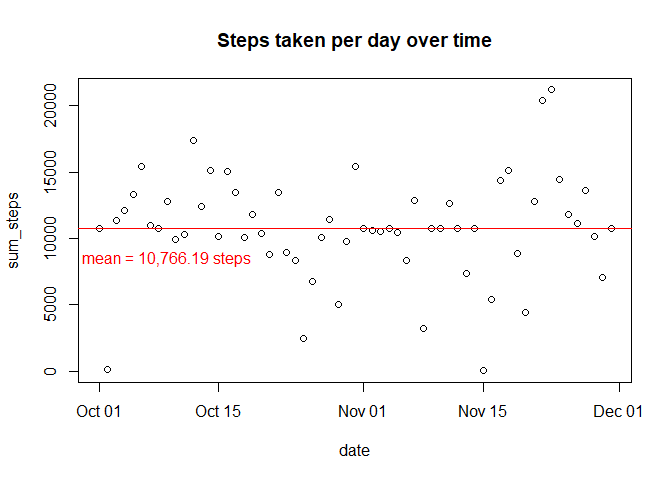
\includegraphics{PA1_template_files/figure-latex/unnamed-chunk-5-1.pdf}

Above, the scatter plot over time shows that there are not obvious
patterns in the time series. On average, the number of steps taken per
day is \textbf{10,766.19} steps. Whereas, the median is
\textbf{10,766.19} steps. Looking at the histogram below, we can see
that the distribution tends to aggregate at the mean and taper off.

\begin{Shaded}
\begin{Highlighting}[]
\CommentTok{# plot histogram for total steps per day}
\NormalTok{h <-}\StringTok{ }\KeywordTok{hist}\NormalTok{(sum_by_date}\OperatorTok{$}\NormalTok{sum_steps, }\DataTypeTok{breaks =} \DecValTok{15}\NormalTok{, }\DataTypeTok{xlab =} \StringTok{"Daily steps"}\NormalTok{, }\DataTypeTok{ylab =} \StringTok{"Count (step)"}\NormalTok{, }
     \DataTypeTok{main =} \StringTok{"Histogram of the total steps taken per day"}\NormalTok{)}


\NormalTok{g <-}\StringTok{ }\NormalTok{sum_by_date}\OperatorTok{$}\NormalTok{sum_steps}
\NormalTok{xfit <-}\StringTok{ }\KeywordTok{seq}\NormalTok{(}\KeywordTok{min}\NormalTok{(g), }\KeywordTok{max}\NormalTok{(g), }\DataTypeTok{length =} \DecValTok{40}\NormalTok{) }
\NormalTok{yfit <-}\StringTok{ }\KeywordTok{dnorm}\NormalTok{(xfit, }\DataTypeTok{mean =} \KeywordTok{mean}\NormalTok{(g), }\DataTypeTok{sd =} \KeywordTok{sd}\NormalTok{(g)) }
\NormalTok{yfit <-}\StringTok{ }\NormalTok{yfit }\OperatorTok{*}\StringTok{ }\KeywordTok{diff}\NormalTok{(h}\OperatorTok{$}\NormalTok{mids[}\DecValTok{1}\OperatorTok{:}\DecValTok{2}\NormalTok{]) }\OperatorTok{*}\StringTok{ }\KeywordTok{length}\NormalTok{(g) }

\KeywordTok{lines}\NormalTok{(xfit, yfit, }\DataTypeTok{col =} \StringTok{"black"}\NormalTok{, }\DataTypeTok{lwd =} \DecValTok{2}\NormalTok{)}
\KeywordTok{abline}\NormalTok{(}\DataTypeTok{v =} \KeywordTok{mean}\NormalTok{(sum_by_date}\OperatorTok{$}\NormalTok{sum_steps),}\DataTypeTok{lwd=}\DecValTok{5}\NormalTok{, }\DataTypeTok{col=}\StringTok{"red"}\NormalTok{)}
\end{Highlighting}
\end{Shaded}

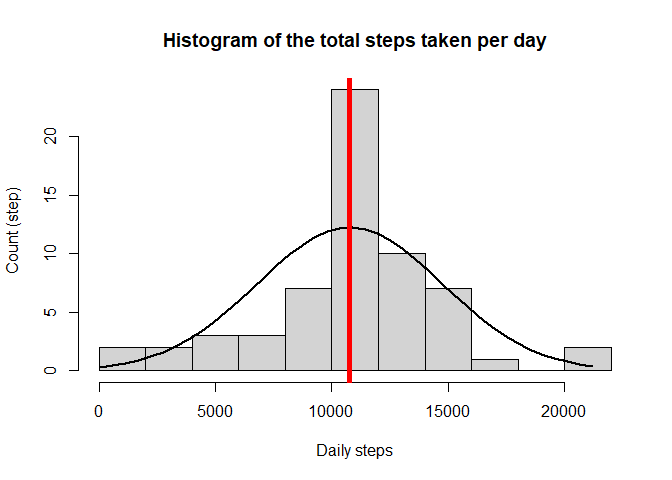
\includegraphics{PA1_template_files/figure-latex/unnamed-chunk-6-1.pdf}

Another interesting thing to look at is whether the day of week makes
any difference to the number of steps taken on average. However, we can
see here that there is no consistent and significant difference between
the number of steps walked based on day of week. In other word, there
are no differences between activities during weekdays and weekends.

\begin{Shaded}
\begin{Highlighting}[]
\CommentTok{# Summarize data by day of week (DOW)}
\NormalTok{sum_by_dow <-}\StringTok{ }\NormalTok{data }\OperatorTok\StringTok{ }
\StringTok{                }\KeywordTok{group_by}\NormalTok{(date) }\OperatorTok\StringTok{ }
\StringTok{                }\KeywordTok{summarize}\NormalTok{(}\DataTypeTok{sum_steps =} \KeywordTok{sum}\NormalTok{(steps))}
\NormalTok{sum_by_dow}\OperatorTok{$}\NormalTok{dow =}\StringTok{ }\KeywordTok{format}\NormalTok{(sum_by_dow}\OperatorTok{$}\NormalTok{date, }\DataTypeTok{format =} \StringTok{"%a"}\NormalTok{)}
\NormalTok{sum_by_dow}\OperatorTok{$}\NormalTok{dow <-}\StringTok{ }\KeywordTok{factor}\NormalTok{(sum_by_dow}\OperatorTok{$}\NormalTok{dow, }\DataTypeTok{levels =} \KeywordTok{c}\NormalTok{(}\StringTok{"Mon"}\NormalTok{, }\StringTok{"Tue"}\NormalTok{, }\StringTok{"Wed"}\NormalTok{, }\StringTok{"Thu"}\NormalTok{, }\StringTok{"Fri"}\NormalTok{, }\StringTok{"Sat"}\NormalTok{, }\StringTok{"Sun"}\NormalTok{))}

\CommentTok{# plot histogram for total steps per day}
\KeywordTok{boxplot}\NormalTok{(sum_steps}\OperatorTok{~}\NormalTok{dow, sum_by_dow, }\DataTypeTok{xlab =} \StringTok{"Day of week"}\NormalTok{, }\DataTypeTok{ylab =} \StringTok{"Sum count (step)"}\NormalTok{, }
     \DataTypeTok{main =} \StringTok{"Box plot of the total steps per day, group by day of week"}\NormalTok{)}
\end{Highlighting}
\end{Shaded}

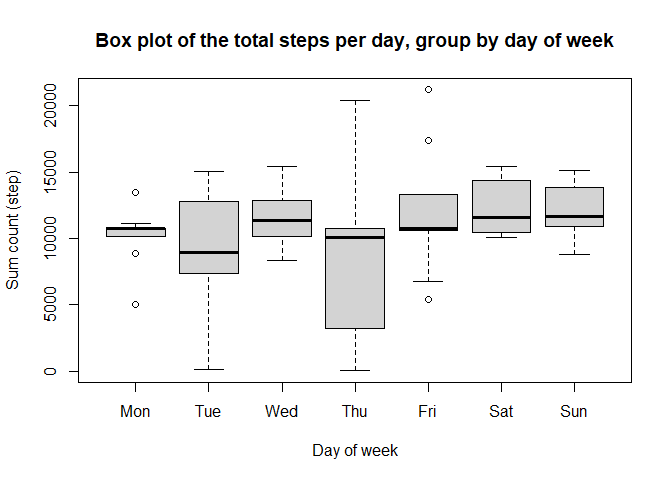
\includegraphics{PA1_template_files/figure-latex/unnamed-chunk-7-1.pdf}

\begin{Shaded}
\begin{Highlighting}[]
\CommentTok{# Summarize data by date}
\NormalTok{sum_by_interval <-}\StringTok{ }\NormalTok{data }\OperatorTok\StringTok{ }
\StringTok{                }\KeywordTok{group_by}\NormalTok{(interval) }\OperatorTok\StringTok{ }
\StringTok{                }\KeywordTok{summarize}\NormalTok{(}\DataTypeTok{sum_steps =} \KeywordTok{sum}\NormalTok{(steps))}

\CommentTok{# plot histogram for total steps per day}
\KeywordTok{barplot}\NormalTok{(sum_steps}\OperatorTok{~}\NormalTok{interval, sum_by_interval, }
        \DataTypeTok{xlab =} \StringTok{"Intervals"}\NormalTok{, }\DataTypeTok{ylab =} \StringTok{"Total number of steps (step)"}\NormalTok{, }
        \DataTypeTok{main =} \StringTok{"Bar plot of 5-minute intervals"}\NormalTok{)}
\end{Highlighting}
\end{Shaded}

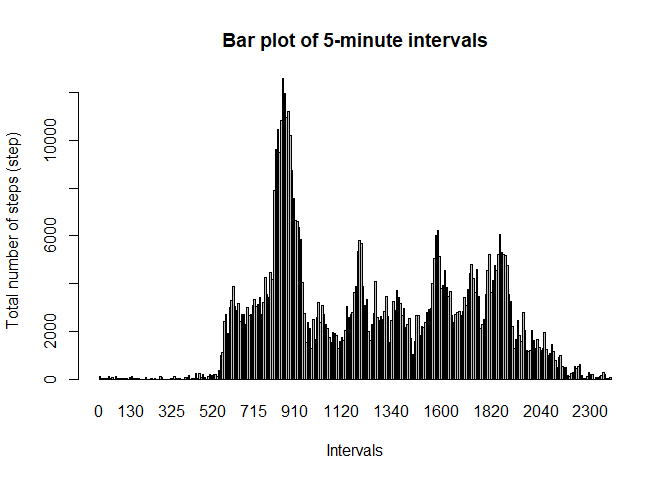
\includegraphics{PA1_template_files/figure-latex/unnamed-chunk-8-1.pdf}

The bar plot above showing the peak interval being \textbf{835.00}
interval.

\end{document}
